%============================================================================%
%
%	DOCUMENT DEFINITION
%
%============================================================================%

%we use article class because we want to fully customize the page and dont use a cv template
\documentclass[10pt,A4]{article}	


%----------------------------------------------------------------------------------------
%	ENCODING
%----------------------------------------------------------------------------------------

%we use utf8 since we want to build from any machine
\usepackage[utf8]{inputenc}		

%----------------------------------------------------------------------------------------
%	LOGIC
%----------------------------------------------------------------------------------------

% provides \isempty test
\usepackage{xifthen}

%----------------------------------------------------------------------------------------
%	FONT
%----------------------------------------------------------------------------------------

% some tex-live fonts - choose your own

% \usepackage[defaultsans]{droidsans}
% \usepackage[default]{comfortaa}
% \usepackage{cmbright}
% \usepackage[default]{raleway}
% \usepackage{fetamont}
\usepackage[default]{gillius}
% \usepackage[light,math]{iwona}
% \usepackage[thin]{roboto} 

% set font default
\renewcommand*\familydefault{\sfdefault} 	
\usepackage[T1]{fontenc}

% more font size definitions
\usepackage{moresize}		

\usepackage{fontawesome5}

%----------------------------------------------------------------------------------------
%	PAGE LAYOUT  DEFINITIONS
%----------------------------------------------------------------------------------------

%debug page outer frames
%\usepackage{showframe}			


%define page styles using geometry
\usepackage[a4paper]{geometry}		

% for example, change the margins to 2 inches all round
\geometry{top=1cm, bottom=-.6cm, left=0.4cm, right=1cm} 	


%less space between header and content
\setlength{\headheight}{-5pt}		

%indentation is zero
\setlength{\parindent}{0mm}

%----------------------------------------------------------------------------------------
%	TABLE /ARRAY DEFINITIONS
%---------------------------------------------------------------------------------------- 

%for layouting tables
\usepackage{multicol}			
\usepackage{multirow}

%extended aligning of tabular cells
\usepackage{array}

\newcolumntype{x}[1]{%
>{\raggedleft\hspace{0pt}}p{#1}}%


%----------------------------------------------------------------------------------------
%	GRAPHICS DEFINITIONS
%---------------------------------------------------------------------------------------- 

%for header image
\usepackage{graphicx}

%for floating figures
\usepackage{wrapfig}
\usepackage{float}
%\floatstyle{boxed} 
%\restylefloat{figure}

%for drawing graphics		
\usepackage{tikz}				
\usetikzlibrary{shapes, backgrounds,mindmap, trees}


%----------------------------------------------------------------------------------------
%	Color DEFINITIONS
%---------------------------------------------------------------------------------------- 
\usepackage{transparent}
\usepackage{color}

%accent color
\definecolor{complcol}{RGB}{250,150,10}

%dark background color
\definecolor{bgcol}{RGB}{110,110,110}

%light background / accent color
\definecolor{softcol}{RGB}{225,225,225}

\definecolor{sectcol}{RGB}{0,120,150}


%Package for links, must be the last package used
\usepackage[hidelinks]{hyperref}

%============================================================================%
%
%
%	DEFINITIONS
%
%
%============================================================================%

% returns minipage width minus two times \fboxsep
% to keep padding included in width calculations
\newcommand{\mpwidth}{\linewidth-\fboxsep-\fboxsep}
	

%----------------------------------------------------------------------------------------
% 	ARROW GRAPHICS in Tikz
%----------------------------------------------------------------------------------------

% a six pointed arrow poiting to the left
\newcommand{\tzlarrow}{(0,0) -- (0.2,0) -- (0.3,0.2) -- (0.2,0.4) -- (0,0.4) -- (0.1,0.2) -- cycle;}	

% include the left arrow into a tikz picture
% param1: fill color
%
\newcommand{\larrow}[1]
{\begin{tikzpicture}[scale=0.58]
	 \filldraw[fill=#1!100,draw=#1!100!black]  \tzlarrow
 \end{tikzpicture}
}

% a six pointed arrow poiting to the right
\newcommand{\tzrarrow}{ (0,0.2) -- (0.1,0) -- (0.3,0) -- (0.2,0.2) -- (0.3,0.4) -- (0.1,0.4) -- cycle;}

% include the right arrow into a tikz picture
% param1: fill color
%
\newcommand{\rarrow}
{
\begin{tikzpicture}[scale=0.7]
	\filldraw[fill=sectcol!100,draw=sectcol!100!black] \tzrarrow
 \end{tikzpicture}
}

%----------------------------------------------------------------------------------------
%	custom sections
%----------------------------------------------------------------------------------------

% create a coloured box with arrow and title as cv section headline
% param 1: section title
%
\newcommand{\cvsection}[1]
{
\colorbox{sectcol}{\mystrut \makebox[1\mpwidth][l]{
\larrow{bgcol} \hspace{-8pt} \larrow{bgcol} \hspace{-8pt} \larrow{bgcol} \textbf{\textcolor{white}{\uppercase{#1}}}\hspace{4pt}
}}\\
}

% create a coloured arrow with title as cv meta section section
% param 1: meta section title
%
\newenvironment{metasection}[1] {
	\vspace{6pt}
	\begin{center}
		\textcolor{white}{\large{\uppercase{#1}}}\\
	\normalsize
	\parbox{0.7\mpwidth}{\textcolor{white}	\hrule}
}{\end{center}}

%----------------------------------------------------------------------------------------
%	 CV EVENT
%----------------------------------------------------------------------------------------

% creates a stretched box as cv entry headline followed by some paragraphs about 
% the work you did
% param 1:	event time i.e. 2014 or 2011-2014 etc.
% param 2:	event name (what did you do?)
% param 3:	institution (where did you work / study)
% param 4:	list of paragraphs outlining your contributions, see example usage below
%
\newcommand{\cvevent}[4]
{
\vspace{6pt}
	\begin{tabular*}{1\mpwidth}{p{0.55\mpwidth}  x{0.42\mpwidth}}
 	\textcolor{black}{\textbf{#2}} & \textcolor{complcol}{#3}, \textcolor{bgcol}{#1} 
	\end{tabular*}
\vspace{0pt}
\textcolor{softcol}{\hrule}
\vspace{6pt}
	\cvlist {#4}
\vspace{-6pt}
}

% formats a list of strings with variable length for use in `\cvevent`
% param 1: a list of strings outlining your contributions
\newcommand{\cvlist}[1] {
    \foreach \listitem in {#1}
    {
        \begin{tabular*}
            {1\mpwidth}{p{1.2\mpwidth}}
            \parbox{1\mpwidth}{\larrow{softcol} \listitem}
            \vspace{3pt}
        \end{tabular*}
    }
}

% creates a stretched box as 
\newcommand{\cveventmeta}[2]
{
	\mbox{\mystrut \hspace{87pt}\textit{#1}}\\
	#2
}

%----------------------------------------------------------------------------------------
% CUSTOM STRUT FOR EMPTY BOXES
%----------------------------------------- -----------------------------------------------
\newcommand{\mystrut}{\rule[-.3\baselineskip]{0pt}{\baselineskip}}

%----------------------------------------------------------------------------------------
% CUSTOM LOREM IPSUM
%----------------------------------------------------------------------------------------
\newcommand{\lorem}
{Lorem ipsum dolor sit amet, consectetur adipiscing elit. Donec a diam lectus.}


% use to vertically center content
% credits to: http://tex.stackexchange.com/questions/7219/how-to-vertically-center-two-images-next-to-each-other
\newcommand{\vcenteredinclude}[1]{\begingroup
\setbox0=\hbox{\includegraphics{#1}}%
\parbox{\wd0}{\box0}\endgroup}

% use to vertically center content
% credits to: http://tex.stackexchange.com/questions/7219/how-to-vertically-center-two-images-next-to-each-other
\newcommand*{\vcenteredhbox}[1]{\begingroup
\setbox0=\hbox{#1}\parbox{\wd0}{\box0}\endgroup}

%----------------------------------------------------------------------------------------
%	ICON-SET EMBEDDING
%---------------------------------------------------------------------------------------- 

% at this point we simplify our icon-embedding by simply referring to a set of png images.
% if you find a good way of including svg without conflicting with other packages you can
% replace this part
\newcommand{\icon}[3]{\makebox(#2, #2){\textcolor{#3}{\csname fa#1\endcsname}}}	%icon shortcut
\newcommand{\icontext}[4]{ 						%icon with text shortcut
	\vcenteredhbox{\icon{#1}{#2}{#4}} \vcenteredhbox{\textcolor{#4}{#3}}
}
\newcommand{\iconhref}[5]{ 						%icon with website url
    \vcenteredhbox{\icon{#1}{#2}{#5}} \href{#4}{\textcolor{#5}{#3}}
}

\newcommand{\iconemail}[5]{ 						%icon with email link
    \vcenteredhbox{\icon{#1}{#2}{#5}} \href{mailto:#4}{\textcolor{#5}{#3}}
}



%============================================================================%
%
%
%
%	DOCUMENT CONTENT
%
%
%
%============================================================================%
\begin{document}
\fcolorbox{white}{white}{\begin{minipage}[c][0.97\textheight][t]{0.69\linewidth}


		%---------------------------------------------------------------------------------------
		%	TITLE HEADLINE
		%----------------------------------------------------------------------------------------
		\vspace{-3pt}
		% use this for multiple words like working titles etc.
		\colorbox{bgcol}{\makebox[\mpwidth][c]{\hspace{40pt}\HUGE{\textcolor{white}{\uppercase{Smeers Timothy}} } \textcolor{sectcol}{\rule[-1mm]{1mm}{0.9cm}} \parbox[b]{5cm}{   \large{ \textcolor{white}{{Consultant informatique}}}\\
					\large{ \textcolor{white}{{Développeur logiciels}}}}
			}}

		% use this for single words, e.g. CV or RESUME etc.
		% \colorbox{bgcol}{\makebox[\mpwidth][c]{\HUGE{\textcolor{white}{\uppercase{Smeers Timothy}} } \textcolor{sectcol}{\rule[-1mm]{1mm}{0.9cm}} \HUGE{\textcolor{white}{\uppercase{Resume}} } }}

		%----------------------------------------------------------------------------------------
		%	HEADER IMAGE
		%----------------------------------------------------------------------------------------


		%\hspace{-1.6cm}
		%\includegraphics[trim= 0 250 0 270,clip,width=1\linewidth+3.1cm]{myfoto.jpg}	%trimming relative to image size!
		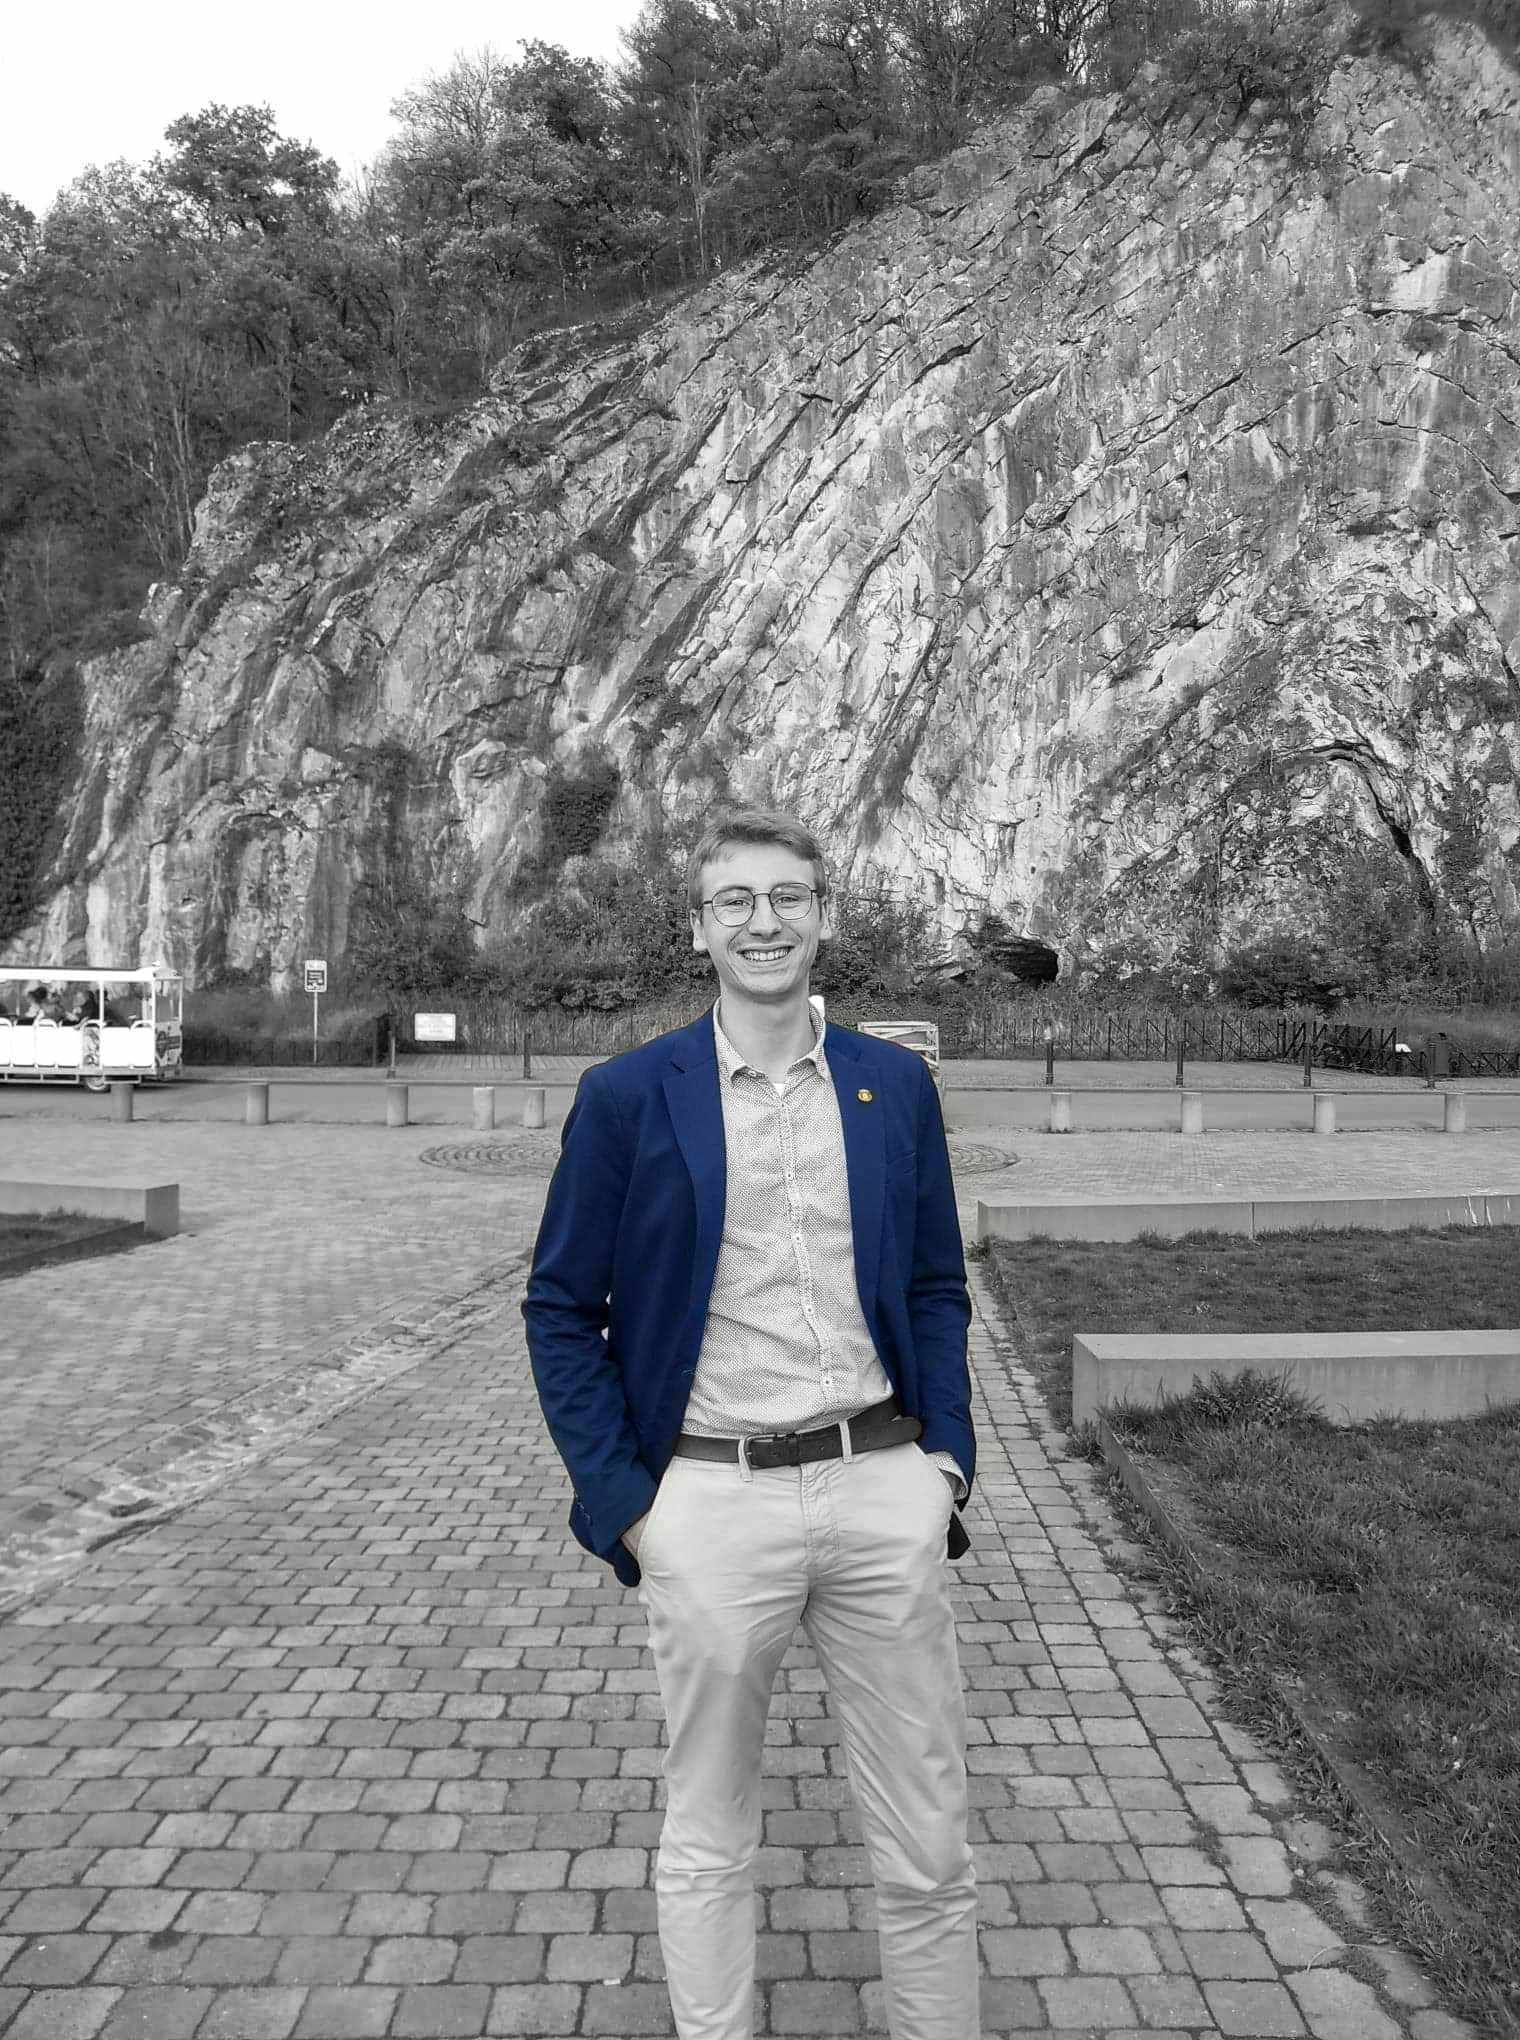
\includegraphics[trim= 490 840 80 800, clip ,width=\linewidth]{Profile.jpg}	%trimming relative to image size

		%---------------------------------------------------------------------------------------
		%	SUMMARY
		%----------------------------------------------------------------------------------------
		\transparent{0.85}%
		\vspace{-140pt}
		\hspace{0.4\linewidth}
		\colorbox{bgcol}{
			\parbox{0.5\linewidth}{
				\transparent{1}%
				\begin{center}
					\larrow{sectcol}\larrow{sectcol}\textcolor{white}{
						Développeur de logiciels spécialisé dans le développement d'applications, bénéficiant d'une solide expérience en programmation acquise à l'Université de Helmo ainsi que dans les systèmes embarqués.}
				\end{center}
			}
		}
		\vspace{60pt}

		%============================================================================%
		%
		%	CV SECTIONS AND EVENTS (MAIN CONTENT)
		%
		%============================================================================%

		%---------------------------------------------------------------------------------------
		%	STATUS
		%----------------------------------------------------------------------------------------
		\cvsection{Statut}
			Développeur de logiciels spécialisé dans le développement d'applications, avec une expertise particulière dans les applications QT et Java.
		\vspace{10pt}

		%---------------------------------------------------------------------------------------
		%	EXPERIENCE
		%----------------------------------------------------------------------------------------
		\cvsection{Expériences}

		\cvevent{2020/05 - maintenant}{Programmeur logiciels}{FlyTek}{développement de tests de validation via l'API Froglogic Squish.,Développement d'applications Qt dans le domaine de la défense.,Diverses tâches Front-end et Back-end.,Création des frameworks CMake et LaTex.,Implémentation d'un ORM SQLite/C++ en utilisant le framework QxORM.}

		%\textcolor{softcol}{\hrule}
		\cvevent{2019/05 - /06}{Erasmus +}{Universidad de Sevilla}{Stage en maintenance de robot bipède dans le cadre d'un projet de Macco Robotics.}

		\vspace{12pt}
		%---------------------------------------------------------------------------------------
		%	EDUCATION SECTION
		%--------------------------------------------------------------------------------------
		\cvsection{Éducation}

		\cvevent{2022 - 2025}{Bachelier Informatique}{Helmo}{Bachelier en développement d'applications. Mes domaines d'expertise comprennent : \\analyste-programmeur{,} développeur d'applications{,} développeur web{,} chef de projet{,} \\ administrateur de base de données{,} consultant en informatique.}

		%\textcolor{softcol}{\hrule}
		\cvevent{2020 - 2022}{Bachelier Science de l'Informatique}{Université de Liège}{Bachelier en Science de l'informatique.}

		%\textcolor{softcol}{\hrule}
		\cvevent{2018 - 2020}{Formations}{Technifutur academy}{BA4{,} BA5{,} VCA, Salle blanche{,} Fiabilité{,} Mécanique{,} Diagnostique de pannes., Hydraulique (proportionnelle){,} Pneumatique (proportionnelle){,} Régulation., Capteur instrumentation{,} Automates programmables.}

		%\textcolor{softcol}{\hrule}
		\cvevent{2019 - 2020}{Électronicien Biomédical}{Athénée Royal d'Esneux}{Maintenance des équipements biomédicaux.,Mémoire : Projet de production de scalpel électrique.,Diplôme en Électronique Biomédicale.}

		%\textcolor{softcol}{\hrule}
		\cvevent{2015 - 2019}{Électronicien}{Athénée Royal d'Esneux}{Certificat d'Enseignement Secondaire Supérieur. Orientation : Électronicien.,Mémoire : Mise en œuvre d'un hexapode suiveur de ligne.,Brevet de Secouriste d'entreprise.,Diplôme d'électricien A2.}
 
	\end{minipage}}%
	\fcolorbox{white}{sectcol}{\begin{minipage}[c][0.97\textheight][t]{0.33\linewidth}


		\begin{metasection}{Contact}

			\icontext{MapMarker}{12}{Liège, Belgique}{white}\\[6pt]
			\icontext{Phone}{12}{+32 478 586 914}{white}\\[6pt]
			\iconhref{MailBulk}{12}{ti.smeers@student.helmo.be}{mailto:ti.smeers@student.helmo.be}{white}\\[6pt]
			\iconhref{Linkedin}{12}{linkedin.com/in/timothy-smeers}{https://www.linkedin.com/in/timothy-smeers-bb59a1189/}{white}\\[6pt]
			\iconhref{Github}{12}{https://github.com/Timothy-Smeers}{https://github.com/Timothy-Smeers}{white}\\[6pt]
			% \iconhref{MousePointer}{12}{http://Timothy-Smeers.com/}{www.Timothy-Smeers.com}{white}\\[6pt]

		\end{metasection}

		%----------------------------------------------------------------------------------------
		%	META SECTION
		%----------------------------------------------------------------------------------------

		\begin{metasection}{Compétences}

			\icontext{}{12}{Implémentation \& Intégration}{white}\\
			\icon{Star}{12}{complcol}\icon{Star}{12}{complcol}\icon{Star}{12}{complcol}\icon{Star}{12}{complcol}\icon{Star}{12}{complcol}\icon{Star}{12}{complcol}\icon{Star}{12}{complcol}\icon{Star}{12}{white}\icon{Star}{12}{white}\icon{Star}{12}{white}\\[6pt]

			\icontext{}{12}{Spécification \& Conception}{white}\\
			\icon{Star}{12}{complcol}\icon{Star}{12}{complcol}\icon{Star}{12}{complcol}\icon{Star}{12}{complcol}\icon{Star}{12}{complcol}\icon{Star}{12}{complcol}\icon{Star}{12}{complcol}\icon{Star}{12}{white}\icon{Star}{12}{white}\icon{Star}{12}{white}\\[6pt]

			\icontext{}{12}{Gestion de projet}{white}\\
			\icon{Star}{12}{complcol}\icon{Star}{12}{complcol}\icon{Star}{12}{complcol}\icon{Star}{12}{complcol}\icon{Star}{12}{complcol}\icon{Star}{12}{complcol}\icon{Star}{12}{white}\icon{Star}{12}{white}\icon{Star}{12}{white}\icon{Star}{12}{white}\\[6pt]


		\end{metasection}


		\begin{metasection}{Technologies}

			\begin{tabular}{ll}
				\textcolor{white}{\icontext{Code}{12}{C/C++}{white}}        & \textcolor{white}{\icontext{Code}{12}{Java}{white}}       \\[6pt]
				\textcolor{white}{\icontext{Code}{12}{Python}{white}}       & \textcolor{white}{\icontext{Code}{12}{LaTeX}{white}}      \\[6pt]
				\textcolor{white}{\icontext{Code}{12}{HTML/CSS/PHP}{white}} & \textcolor{white}{\icontext{Code}{12}{SQL}{white}}        \\[6pt]
				\textcolor{white}{\icontext{Code}{12}{C\#}{white}}          & \textcolor{white}{\icontext{Code}{12}{Kotlin}{white}}     \\[6pt]
				\textcolor{white}{\icontext{Code}{12}{.NET}{white}}         & \textcolor{white}{\icontext{Code}{12}{JavaScript}{white}} \\[6pt]
			\end{tabular}
		\end{metasection}

		\begin{metasection}{Outils}

			\begin{tabular}{ll}
				\textcolor{white}{\icontext{CodeBranch}{12}{Atlassian}{white}}  & \textcolor{white}{\icontext{CodeBranch}{12}{Git}{white}}              \\[6pt]
				\textcolor{white}{\icontext{CodeBranch}{12}{Eclipse}{white}}    & \textcolor{white}{\icontext{CodeBranch}{12}{VsCode}{white}}           \\[6pt]
				\textcolor{white}{\icontext{CodeBranch}{12}{Qt5.15/6.5}{white}} & \textcolor{white}{\icontext{CodeBranch}{12}{QxORM}{white}}            \\[6pt]
				\textcolor{white}{\icontext{CodeBranch}{12}{CMake}{white}}      & \textcolor{white}{\icontext{CodeBranch}{12}{Froglogic Squish}{white}} \\[6pt]
				\textcolor{white}{\icontext{CodeBranch}{12}{MPLAB}{white}}      &
			\end{tabular}
		\end{metasection}

		\begin{metasection}{Systèmes d'exploitation}

			\textcolor{white}{\LARGE{\icon{Linux}{24}{white} \icon{Windows}{24}{white}  \icon{Android}{24}{white}}}

		\end{metasection}
		
		\begin{metasection}{Activités}

			\textcolor{white}{\LARGE{\icon{HorseHead}{24}{white} \icon{Hiking}{24}{white}  \icon{LaptopCode}{24}{white}}}
		\end{metasection}

		%---------------------------------------------------------------------------------------
		%	QR CODE (optional)
		%----------------------------------------------------------------------------------------

		% \vspace{12pt}
		% \begin{center}
		% 	\includegraphics[width=0.35\mpwidth]{qrcode}
		% \end{center}

		%---------------------------------------------------------------------------------------
		%	optional TEXT
		%----------------------------------------------------------------------------------------
		\vspace{73pt}
		\begin{center}
			\textcolor{white}{Passion is everything. In fact, you've got to be borderline fanatical about what you do.}
			% \textcolor{white}{\icontext{CodeBranch}{12}{Ce CV a été rédigé en utilisant \LaTeX}{white}}
		\end{center}

	\end{minipage}}

%-------------------------------------------------------------------------------------------------
%	ARTIFICIAL FOOTER (fancy footer cannot exceed linewidth) 
%--------------------------------------------------------------------------------------------------

\null
% \vspace*{\fill}
\hspace{-0.25\linewidth}\colorbox{bgcol}{\makebox[1.5\linewidth][c]{\mystrut \small \textcolor{white}{Copyright 2024 Smeers Timothy} $\cdot$ \textcolor{white}{ti.smeers@student.helmo.be}}}\\[-10pt]

%============================================================================%
%
%
%
%	DOCUMENT END
%
%
%
%============================================================================%
\end{document}
